\documentclass[]{article}
\usepackage{mathtools}
\usepackage{tikz}
\DeclarePairedDelimiter\floor{\lfloor}{\rfloor}

%opening
\title{Problem session 2}
\author{Dibran Dokter 1047390}

\begin{document}
	
	\maketitle
	
	\section{}
	\subsection{}
	
	n = 0\\
	x = L.head\\
	while x.next != NIL\\
		\null\qquad n+=1\\
		\null\qquad x = x.next\\
	v = $ \floor{n/2)}$\\
	x = head\\
	n = 0\\
	while x.next != NIL\\
		\null\qquad if n == v\\
			\null\qquad\qquad return x.ky\\
		\null\qquad n++\\
		\null\qquad x = x.next\\
		
	\subsection{}
	
	1)\\

	isEmpty()\\
		\null\qquad return no\_elements == 0\\
	
	push(element)\\
		\null\qquad setLength(stack, no\_elements+1)\\
		\null\qquad stack[no\_elements] = element\\
		\null\qquad no\_elements += 1\\
		
	pop()\\
		\null\qquad if isEmpty(stack)\\
		\null\qquad\qquad error "Stack empty"\\
		\null\qquad elem = stack[no\_elements]\\
		\null\qquad setLength(stack, no\_elements-1)\\
		\null\qquad return elem\\
	
	top()\\
		\null\qquad if isEmpty(stack)\\
		\null\qquad\qquad error "Stack empty"\\
		\null\qquad return stack[no\_elements]\\
		
	display()\\
		\null\qquad n = 0\\
		\null\qquad while n $<$ no\_elements\\
		\null\qquad\qquad writeLn(stack[n])\\
		
	2)\\
	
	createStack() =	$\mathcal{O}(1)$\\
	isEmpty() = $\mathcal{O}(1)$\\
	push(element) = $\mathcal{O}(1)$\\
	pop() = $\mathcal{O}(1)$\\
	top() = $\mathcal{O}(1)$\\
	display() = $\mathcal{O}(n)$\\
	
	3)\\
	
	"AAA"\\
	"AAA"\\
	"BBB"\\
	"CCC"\\
	"CCC"\\
	"AAA"\\
	"BBB"\\
	
	4)\\
	
	empty()\\
		\null\qquad setLength(stack,0)\\
		\null\qquad no\_element = 0\\
	
	\subsection{}
	
	when we push n elements after m the time for m is :\\
	$t(m) = y + (n\cdot x) + (n\cdot y) + (n\cdot x) + (n\cdot y) = n \cdot 2XY+y$\\
	because we need the first y between the end of the first push and the next one, then we have (n-1) pushes and pauses to push in the rest of the n elements
	after that we start popping the rest of the elements until we get to the pop of the element m
	
	\subsection{}
	
	\begin{tabular}{|l l|}
		
		\hline
		
		Q:		& 1\\
		$\pi$:	& 1\\
		d:		& 0\\
		
		\hline
		
		Q:		& 2 3 4\\
		$\pi$:	& 1 1 1\\
		d:		& 1 1 1\\
		
		\hline
		
		Q:		& 3 4\\
		$\pi$:	& 1 1\\
		d:		& 1 1\\
		
		\hline
		
		Q:		& 4 5 6\\
		$\pi$:	& 1 3 3\\
		d:		& 1 2 2\\
		
		\hline
		
		Q:		& 5 6\\
		$\pi$:	& 3 3\\
		d:		& 2 2\\
		
		\hline
		
		Q:		& 6\\
		$\pi$:	& 3\\
		d:		& 2\\
		
		\hline
		
	\end{tabular}

	\subsection{}
	
	To solve this we first run BFS and then we find the vertices which have an outgoing edge with s.\\
	If they have an outgoing edge with s and are in the BFS list as connected to s we have found a cycle.\\
	Then we find the shortest cycle using the distance and return the cycle by getting the predecessors from the vertex.\\
	
	\newpage
	
	findShortestCycle(G, s)\\
		\null\qquad bfsList = BFS(G, s)\\
		\null\qquad outGoingVertex = []\\
		\null\qquad foreach v in G\\
		\null\qquad\qquad if(v.neighbor == s)\\
		\null\qquad\qquad\qquad outGoingVertex.push(v)\\
		\null\qquad shortestVertex = s\\
		\null\qquad minDistance = $\infty$\\
		\null\qquad foreach v in outGoingVertex\\
		\null\qquad\qquad if v in bfsList
		\null\qquad\qquad\qquad if v.distance $<$ minDistance\\
		\null\qquad\qquad\qquad\qquad shortestVertex = v\\
		\null\qquad if shortestVertex == s\\
		\null\qquad\quad return False\\
		\null\qquad shortestCycle = []\\
		\null\qquad shortestCycle.push(shortestVertex)\\
		\null\qquad vertex = shortestVertex\\
		\null\qquad while vertex.distance $>$ 0\\
		\null\qquad\qquad shortestCycle.push(vertex.predecessor)\\
		\null\qquad\qquad vertex = vertex.predecessor\\
		\null\qquad return (True, shortestCycle)\\
		
	The algorithm first runs BFS to find the paths to s. Then we find the vertices which go to s.
	
	After that we find the vertices which have both an outgoing connection to s and an incoming connection by checking if the vertex is in the BFS list.
	
	If there is a path from a vertex connected to s back to s we have found a cycle. Otherwise there does not exist a cycle.
	
	When we have found the cycle we add the found vertex and loop through the predecessors in the BSF list to create a list of vertices which form the cycle.
	
	\subsection{}
	
	G has to be a undirected and connected graph.\\
	To solve this we need to see that when a vertex has a neighbor that has another neighbor we can create a cycle.\\
	This will not be a simple cycle since the vertices are not distinct.\\
	
	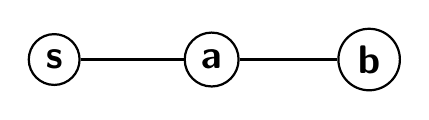
\begin{tikzpicture}[auto, node distance=2cm, every loop/.style={},
	thick,main node/.style={circle,draw,font=\sffamily\Large\bfseries}]
	
	\node[main node] (s) {s};
	\node[main node] (a) [right of=s] {a};
	\node[main node] (b) [right of=a] {b};
	
	  \path[every node/.style={font=\sffamily\small}]
	  
	   (s) edge node {} (a)
	   (a) edge node {} (b);
	
	\end{tikzpicture}
	
	The cycle here is : [s, A, B, A, s].\\
	
	This leads to the algorithm:
	
	isCyclic(G, s)\\
		\null\qquad $foreach\ v \in adj[s]$\\
		\null\qquad\qquad if adj[v] != NIL\\
		\null\qquad\qquad\qquad return True\\
		\null\qquad\qquad else return False\\
	
\end{document}
